\documentclass[11pt]{article}
\usepackage{enumitem}
\usepackage{listings}
\usepackage{tikz}
\usepackage{url}
%\usepackage{algorithm2e}
\usetikzlibrary{arrows,automata,shapes}
\tikzstyle{block} = [rectangle, draw, fill=blue!20, 
    text width=5em, text centered, rounded corners, minimum height=2em]
\tikzstyle{bt} = [rectangle, draw, fill=blue!20, 
    text width=4em, text centered, rounded corners, minimum height=2em]

\lstset{ %
language=Java,
basicstyle=\ttfamily,commentstyle=\scriptsize\itshape,showstringspaces=false,breaklines=true,numbers=left}

\newtheorem{defn}{Definition}
\newtheorem{crit}{Criterion}

\newcommand{\handout}[5]{
  \noindent
  \begin{center}
  \framebox{
    \vbox{
      \hbox to 5.78in { {\bf Software Testing, Quality Assurance and Maintenance } \hfill #2 }
      \vspace{4mm}
      \hbox to 5.78in { {\Large \hfill #5  \hfill} }
      \vspace{2mm}
      \hbox to 5.78in { {\em #3 \hfill #4} }
    }
  }
  \end{center}
  \vspace*{4mm}
}

\newcommand{\lecture}[4]{\handout{#1}{#2}{#3}{#4}{Lecture #1}}
\topmargin 0pt
\advance \topmargin by -\headheight
\advance \topmargin by -\headsep
\textheight 8.9in
\oddsidemargin 0pt
\evensidemargin \oddsidemargin
\marginparwidth 0.5in
\textwidth 6.5in

\parindent 0in
\parskip 1.5ex
%\renewcommand{\baselinestretch}{1.25}

\usepackage{fontspec}
\setmonofont{Cousine}[Scale=MatchLowercase]


\begin{document}

\thispagestyle{empty}
\paragraph{FSM for Question 4.}

\begin{center}
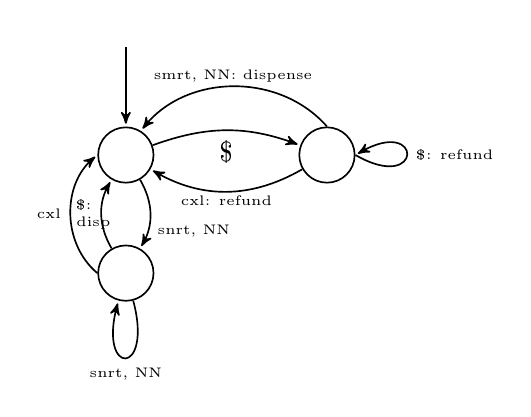
\begin{tikzpicture}[->,>=stealth',shorten >=1pt,auto,node distance=1.5cm,
                    semithick,initial text=]

  \node (0) {};
  \node [minimum size=2em, circle, draw] (1) [below of= 0] {};
  \node [minimum size=2em, circle, draw] (2) [right of= 1, xshift=3em] {};
  \node [minimum size=2em, circle, draw] (3) [below of= 1] {};

  \path (0) edge (1);
  \path (1) edge [bend left=20] node[below] {\$} (2);
  \path (2) edge [bend left] node[yshift=.2em] {\tiny cxl: refund} (1);
  \path (2.north) edge [bend right=50] node[above,yshift=-.2em] {\tiny smrt, NN: dispense} (1);
  \path (2.east) edge [loop right, in=30, out=-30, min distance=10mm] node {\tiny \$: refund} (2.east);

  \path (1) edge [bend left] node[right,near end] {\tiny snrt, NN} (3);
  \path (3) edge [bend left] node[left,xshift=1.5em] {\tiny \begin{minipage}{3em} \$: \\ disp
    \end{minipage}
  } (1);
  \path (3) edge [loop below, min distance=10mm] node {\tiny snrt, NN} (3);
  \path (3.west) edge [bend left=50] node {\tiny cxl} (1.west);

%  \path (1) edge node {} (2)
%        (2) edge node[left] {F} (3)
%            edge [bend left] node {T} (4)
%        (3) edge [bend left] node {} (2.west);
\end{tikzpicture}
\end{center}
\end{document}
